

\chapter{Einleitung}

Das \randbem{Testgetriebene Entwicklung...}Hauptthema dieser Diplomarbeit, die Testgetriebene Entwicklung, ist vielen Programmierern vom Namen her bekannt. Ungeachtet dessen, das  viele Studien über die (positiven) Auswirkungen über diesen Entwicklungsansatz  existieren, so wird sie trotzdem relativ selten eingesetzt, und es existieren große Vorbehalte, wie z.B. dass es Zeitverschwendung sei, oder dass Programmierer fälschlicherweise annehmen, sie könnten die Komplexität überschauen\footnote{\url{http://tamasgyorfi.wordpress.com/tag/excuses-to-tdd/}}.\\
Diese, teilweise mythenumrankte Technik, hat innerhalb des Entwicklerteams der pludoni GmbH ein großes Interesse geweckt, und wird aus diesem nun näher untersucht.

Die \randbem{...von Webserveranwendungen...}pludoni GmbH benötigt für ihre Services gut funktionierende und effizient entwickelte Webserveranwendungen. Das Framework Ruby on Rails scheint dafür wie geschaffen, und erste kleinere Erfahrungen waren durchaus positiv. Durch eine vielbestätigte effektive Entwicklung ist Rails ideal für den Einsatz in kleinen Teams, wie das Entwicklerteam der pludoni GmbH eines ist.

Dieses Framework \randbem{...auf Basis von Ruby on Rails} ist das zweite große Thema dieser Diplomarbeit. Rails und Testen passen anscheinend sehr gut zusammen, da das Testen im Allgemeinen in der Ruby-Community einen sehr hohen Stellenwert hat. Außerdem existiert eine Vielzahl von Testwerkzeugen und die meisten bekannten Bibliotheken verfügen über ausgiebige Tests. Damit passen die Testgetriebene Entwicklung und Ruby (on Rails) perfekt zusammen.

Um die Auswirkungen der Testgetriebenen Entwicklung besser nachzuvollziehen können, benötigt man ein Messinstrument. Dafür sind in diesem Kontext der Webentwicklung die Code-Metriken geeignet. Sie können einen groben Überblick über den Zustand des Quellcodes geben. Daher sind sie ideal, inbesondere in der Lernphase der Testgetriebenen Entwicklung Feedback zu geben.

Wie das Zusammenspiel von Ruby (on Rails), der Testgetriebenen Entwicklung und der Einsatz von Code-Metriken praktisch erfolgen, wird in dieser Arbeit im Detail betrachtet und mit eigenen praktischen Erfahrungen belegt.

\section{Motivation}

Kurz nach der Firmengründung der pludoni GmbH absolvierte der Autor dort sein Pflichtpraktikum, und war danach weiterhin als Werkstudent tätig.
Während dieser Zeit nahmen Programmierer verschiedener Erfahrungsstufen und auch Praktikanten an der Neu- und Weiterentwicklung der Webserversoftware teil. Dies hat zur Folge, dass die Komplexität der Software inzwischen ein Level erreicht hat, bei dem das Maß an Regressionsfehlern\footnote{fehlerauslösender Quelltextänderungen} stark anstieg.

Da zum großen Teil keine automatisierten Softwaretests geschrieben wurden, lassen sich diese nur schwer auffinden. Ein Versuch, nachträglich Softwaretests hinzuzufügen wurde evaluiert und als zu aufwändig befunden, da der Code in seinem jetzigen Zustand nur äußerst schwer zu testen ist. Gründe dafür sind suboptimale Codestrukturen (Spaghetticode), die schwer bis unmöglich zu testen sind. Hier müsste zuerst refaktorisiert werden, aber da keine Tests vorhanden sind, ist dies aufgrund der Regressionsfehler riskant. %Ein Teufelskreis!

Für ein neues Projekt, it-jobs-und-stellen.de, soll dies nun mit einem anderen Ansatz verlaufen.

Neben der Umstellung auf ein modernes Web-Framework sollen nun Tests im Einklang zum Code erstellt werden, um auf Knopfdruck  umfassende Informationen über den Systemzustand zu erhalten, wie sie ein manueller Test in der Gründlichkeit und Schnelligkeit niemals erreichen kann. Außerdem besteht die Hoffnung auf eine nachhaltige Verbesserung der Code-Qualität, um in Zukunft flexibel auf Änderungen reagieren zu können.


\subsection{Die pludoni GmbH}

Die pludoni GmbH ist ein junges dynamisches Dresdner Unternehmen, dass sich zum Ziel gesetzt hat, lokale Communitys zur gegenseitigen Fachkräfteempfehlung aufzubauen und zu betreuen, sowie Tools für die Vereinfachung der Personalarbeit mittelständischer Unternehmen zu entwickeln. Einige Beispiele für diese Communitys sind zur Zeit ITsax.de, ITmitte.de und MINTsax.de\footnote{http://www.itsax.de/, http://www.itmitte.de, http://www.mintsax.de/}.
\marginline{
\includegraphics[width=0.8\marginparwidth]{material/pludoni.png}\\\centering pludoni GmbH}
\paragraph{Funktionsweise der Communitys}
Die Communitys bestehen jeweils aus einer Anzahl mittelständischer Unternehmen einer Branche, Bildungseinrichtungen sowie Vertetern von Städten und Vereinen. Für ITsax.de ist das die IT-Branche. Neben diesem Branchenfokus sammeln sich nur Unternehmen einer spezifischen Region. Bei ITsax.de ist dies Mittel- und Ostsachsen, bei ITmitte.de z.B. Mitteldeutschland, d.h. Thüringen, Sachsen-Anhalt und Westsachsen.
\begin{table}[htbp]
\label{tb:dt}
\caption{Übersicht über pludoni Communitys. Stand September 2011}
\begin{tabular}{|l|p{3.8cm}|p{5cm}|l|}
\hline
\rowcolor{Gray}
Community & Branche & Region & Mitglieder \\\hline
ITsax.de & IT, Software &  Sachsen (Fokus Süden und Osten) & 63\\\hline
ITmitte.de & IT, Software &  Mitteldeutschland (Thüringen, Sachsen-Anhalt, Westsachsen) & 57 \\\hline
MINTsax.de & Maschinenbau, Elektrotechnik &  Sachsen & 29\\\hline
OFFICEsax.de & Vertrieb, Bürotätigkeiten &  Sachsen & in Vorb.\\\hline
OFFICEmitte.de & Vertrieb, Bürotätigkeiten &  Mitteldeutschland & in Vorb.\\\hline
\end{tabular}
\end{table}



Diese Unternehmen, die einen jährlichen Mitgliedsbeitrag für das Community\hyp{}Management\footnote{Ein Überblick über die Aufgaben eines Community-Managers finden Sie unter \url{http://www.pludoni.de/leistungen}} und Weiterentwicklung der Portale an die pludoni GmbH zahlen, dürfen Ihre für die Region relevanten Jobangebote auf dem jeweiligen Portal einstellen. Was die Communitys von pludoni von der dem bisherigen Online-Jobbörsen unterscheidet, ist das sogenannte \textbf{Empfehlungssystem}.

\begin{figure}[htbp]
 \centering
 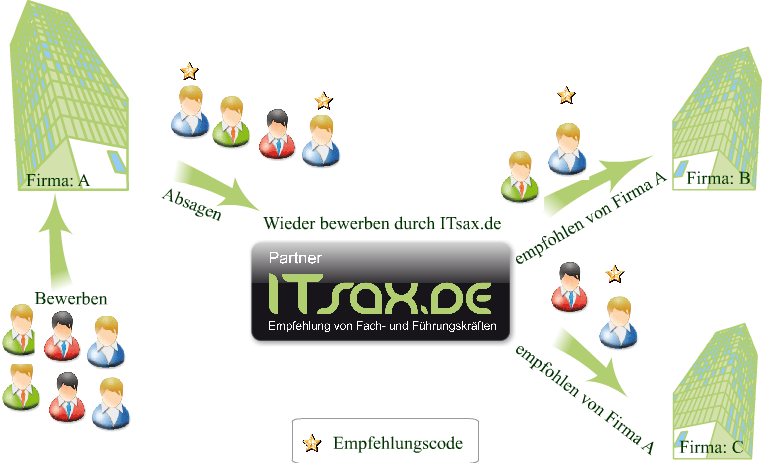
\includegraphics[width=0.8\textwidth]{./material/empfehlungscode.png}
 % empfehlungscode.png: 762x463 pixel, 72dpi, 26.88x16.33 cm, bb=0 0 762 463
 \caption{Funktionsweise des Empfehlungscodes}
 \label{fig:empfehlung}
\end{figure}
Viele der Personalmitarbeiter der beteiligten Firmen haben dieselbe Erfahrung gemacht, dass sie sehr guten Bewerbern absagen mussten, weil z.B. die Stelle schon vergeben wurde, die Fähigkeiten des Bewerbers nicht den Bedürfnissen des Unternehmens entsprachen, oder andere äußere Widrigkeiten eine Einstellung verhinderten. Hier setzt pludoni mit seinen Communitys an, und stellt eine Infrastrukur zur gegenseitigen Empfehlung dieser guten Bewerber bereit.  Ausgezeichnete Bewerber erhalten neben der Absage einen Empfehlungscode, mit dem sie sich auf dem Online-Jobportal bei einer der anderen Mitgliedsfirmen bewerben können, vgl. Abbildung \ref{fig:empfehlung}. Die Software löst intern den Empfehlungscode auf und bestätigt dieser Firma nun, dass der Bewerber von einem anderen Unternehmen der Community empfohlen wurde.

Dieses Empfehlungssystem überzeugt die beteiligten Unternehmen. Aktuell wurden im letzten Jahr z.B. auf ITmitte.de über 800 Bewerberungen über das Portal versendet, von denen mehr als die Hälfte (440) mit Empfehlungscodes versehen waren \citep{joerg_klukas_startseite_2011}. Dies motivierte mittlerweile über 150 Organisationen bei den drei pludoni Communitys teilzunehmen \citep{joerg_klukas_referenzen_2011}.

\subsection{Arbeitsablauf in der pludoni GmbH}
\label{sec:arbeitsablauf}
Die pludoni GmbH stellt sich dem Trend der Dezentralisierung von Arbeit, um einerseits Kundenwünsche zur individuellen Betreuung und andererseits Mitarbeiterwünsche nach flexiblen und familienfreundlichen Arbeitsplätzen gerecht zu werden. Ein Großteil der Arbeit findet somit vor Ort beim Kunden, oder in Heim- / Telearbeit statt.
Zur persönlichen Abstimmung findet aber mindestens einmal pro Woche ein Meeting statt, in welchem sich 2-4 der Mitarbeiter treffen, um alte Aufgaben abzunehmen und Neue zu diskutieren. Die Abnahme erfolgt dabei durch den Teamleiter des Projekts oder dem Geschäftsführer Jörg Klukas.

Zentrales Kommunikationsmittel der pludoni GmbH ist, neben der E-Mail, die Online-Aufgaben- und Fehlerverwaltung Redmine\footnote{\url{http://www.redmine.org} -- ein webbasiertes Projektmanagement-Tool auf der Basis von Ruby on Rails. Redmine kann für Benutzer- und Projektverwaltung, Diskussionsforen, Wikis, zur Ticketverwaltung oder Dokumentenablage genutzt werden, \textit{Wikipedia}}. Dort werden alle Aufgaben und Fehler erfasst und an die zuständigen Personen verteilt.
Neben den technischen Aufgaben der Entwickler werden auch nicht-technische Aufgaben der anderen Mitarbeiter verwaltet, wie z.B. die Gewinnung neuer Partner (Akquise) oder administrative Aufgaben.

Trotz dieses Tools und Vorgehensweise ist die dezentrale Kollaboration aber immer mit Nachteilen in der Kommunikation behaftet. Dies hat bei den Programmierern teils gravierende Auswirkungen auf die Produktivität. Einerseits, da gleiche Funktionalität doppelt implementiert wird, weil der Überblick fehlt, und somit unnötigerweise neue Fehlerquellen eröffnet werden. Andererseits, weil aufgrund der zeitlich asynchronen Arbeitsleistungen Rückmeldungen der anderen Programmierer oder ein Code-Audit nicht immer gewährleistet werden und Regressionsfehler nicht abgeschätzt werden können, da nicht alle Module bekannt sind.


Für das kommende Projekt soll nun eine großflächige Testinfrastruktur erstellt werden, um eine aktuelle Dokumentation des Quelltextes zu erhalten und die Code-Qualität verbessern und natürlich um das Risiko für Regressionsfehler zu minimieren.
